% Using KOMA Script document style
% Font size setting and
% option to skip empty lines as new paragraphs
\documentclass[10pt,a4paper]{article}
% Packages without Options
\usepackage{
	algorithm,
	alltt,
	algpseudocode,
	amsfonts,
	amssymb,
	appendix,
	array,
	booktabs,
	dirtree,
	enumitem,
	float,
	footnote,
	gensymb,
	geometry,
	graphicx,
	interval,
	karnaugh-map,
	lipsum,
	listings,
	longtable,
	makecell,
	mathtools,
	minted,
  nicematrix,
	parskip,
	pdfpages,
	pgfkeys,
	pgfplots,
	subcaption,
	tabularx,
	tablefootnote,
	textcomp,
	tikz,
    titlecaps,
	venndiagram,
	wrapfig,
	wrapfig,
	xcolor
}



% Packages with Options

\usepackage[framemethod=tikz]{mdframed}
\usepackage[colorlinks,linkcolor=cyan, citecolor=cyan, urlcolor=cyan]{hyperref}
\usepackage[labelfont=bf,textfont=it,labelsep=period]{caption}
\usepackage[RPvoltages]{circuitikz}
\usepackage[english]{babel}
\usepackage[nameinlink,noabbrev]{cleveref}

\definecolor{mintedbackground}{rgb}{0.97,0.97,0.97}

\setminted[cpp]{
bgcolor=mintedbackground,
    linenos=true,
    breaklines=true,}

\setminted[js]{
bgcolor=mintedbackground,
    linenos=true,
    breaklines=true,}

\setminted[python]{
bgcolor=mintedbackground,
    linenos=true,
    breaklines=true,}
    

\linespread{1.5}

% Package: AlgorithmicX
% Sets all comments to be indentend and aligned

\renewcommand{\Comment}[2][.7\linewidth]{%
  \leavevmode\hfill\makebox[#1][l]{//~#2}}


% Package: Interval
% Sets the style of mathematical intervals
\intervalconfig{
soft open fences, separator symbol=,,
}

% Package: Geometry
% Sets the page margins
\geometry{
    a4paper,
    left=32mm,
    right=22mm,
    top=22mm,
    }
	
% Creates a proper caption name for algorithms
\newcommand{\algorithmautorefname}{Algorithm}
\newcommand{\listingautorefname}{Listing}
\algrenewcommand{\algorithmiccomment}[1]{\texttt{// #1} }
% Creates a numbered environment for Theorems
\newtheorem{theorem}{Theorem}

% Redefine the implication arrow to be a simple, thin arrow instead of the default, thick arrow
\renewcommand{\implies}{\rightarrow}

% Create a new command for the set complement to make my logical statements easier to read
\newcommand{\compl}{\overline}

% Creates commands for combinatorics nCr and nPr
\newcommand{\nCr}[2]{\,_{#1}C_{#2}} % nCr
\newcommand{\nPr}[2]{\,_{#1}P_{#2}} % nPr

% Package: tikz
% Loads libraries for drawing automata, 
\usetikzlibrary{automata,positioning,shadows,arrows, shapes.gates.logic.US, calc}

% Creates a command to create a button shape
\newcommand*\keystroke[1]{%
  \tikz[baseline= (key.base)]
    \node[%
      draw,
      fill=white,
      drop shadow={shadow xshift=0.25ex,shadow yshift=-0.25ex,fill=black,opacity=0.75},
      rectangle,
      rounded corners=2pt,
      inner sep=1pt,
      line width=0.5pt,
      font=\scriptsize\sffamily
    ] (key) {#1\strut};
}

% Package: pgfplot
% Sets the global options for PGF Plots
\pgfplotsset{compat=newest}

% Package: tikz
% Flowchart Shapes
\tikzstyle{startstop} = [rectangle, rounded corners, minimum width=3cm, minimum height=1cm,text centered, draw=black, fill=red!30]
\tikzstyle{io} = [trapezium, trapezium left angle=70, trapezium right angle=110, minimum width=3cm, minimum height=1cm, text centered, draw=black, fill=blue!30]
\tikzstyle{process} = [rectangle, minimum width=3cm, minimum height=1cm, text centered, draw=black, fill=orange!30]
\tikzstyle{decision} = [diamond, minimum width=3cm, minimum height=1cm, text centered, draw=black, fill=green!30]
\tikzstyle{arrow} = [thick,->,>=stealth]

% Disable Minted syntax error highlights (red boxes)
\AtBeginEnvironment{minted}{%
  \renewcommand{\fcolorbox}[4][]{#4}}

% Listings Style (non-minted)

\lstdefinestyle{arjuncode}{
    basicstyle=\ttfamily,
    breakatwhitespace=false,         
    breaklines=true,                 
    captionpos=b,                    
    keepspaces=true,                 
    numbers=left,                    
    numbersep=5pt,                  
    showspaces=false,                
    showstringspaces=false,
    showtabs=false,                  
    tabsize=2
}

\lstset{style=arjuncode}

\graphicspath{{images/}}

 %Adjust this based on where your Summary is stored
\title{CM3020: Artificial Intelligence \\ Midterm Assignment}
\author{Arjun Muralidharan}
\begin{document}

\maketitle
\newpage
\tableofcontents
\listoffigures
\listoftables
% \listofalgorithms

\newpage
\renewcommand{\subsubsectionautorefname}{section\negthinspace}

\section{Part A: Reviewing research papers about robotic science}

\subsection{Introduction to the field of robotic science}
Robotic science is a field describing agents that can ``automatically originate hypotheses to explain observations, devise experiments to test these hypotheses, physically run the experiments by using laboratory robotics, interpret the results, and then repeat the cycle'' \cite{king_automation_2009}. It aimes to formalize scientific discovery in mathematical terms, so that it can be automated as a process. This way, scientific research can be automated and reproduced more easily. Recent efforts include the use of active learning and deep learning techniques.

\subsection{Descriptions of three papers about robotic science}

\subsubsection{Integrating Quantitative and Qualitative Discovery: The ABACUS System}
In \cite{falkenhainer_integrating_1986}, the researchers attempt at combining qualitative and quantitative learning methods to build an inductive learning progream that can formulate equations and describe the conditions that need to apply for these equations. It uses the techniques of \textit{units analysis}, \textit{proportionality graph search} and \textit{suspension search} to narrow the search space of equations. The researches evaluated the performance by applying the program to various fields in physics and chemistry.

\subsubsection{Towards Robot Scientists for autonomous scientific discovery}
In \cite{sparkes_towards_2010}, the researchers review the main components of autonomous scientific discovery leading up to the concept of a Robot Scientist. The researches aimed to argue that scientific discovery can be fully formalized in logic, making research more reproducible and reusable. The authors developed a custom ontology to formalise the results from previously built agents (e.g. ADAM or EVE) to evaluate the performance. They go on to formulate an inductive argument in support of automated laboratory technologies.

\subsubsection{Functional genomic hypothesis generation and experimentation by a robot scientist}
In \cite{king_functional_2004}, the authors describe how they used robitic science techniques applied to determination of gene function using deletion mutants of yeast. The researchers attempted to demonstrate that an intelligent agent would be as successful as humans in selecting experiments for hypothesis testing. This work employed the use of learning algorithms \cite{lederberg_applications_1969} and \textbf{active learning} techniques. They evaluated the work using a formula to determine the experiment cost, and compared the cost of experiments against the results between humans and the agent.

\subsection{Creating a timeline}
\paragraph{1969} Learning algorithms for analysis of mass-spectrometric data are proposed in \cite{lederberg_applications_1969} and used in DENDRAL \cite{feigenbaum_artificial_1968}, \cite{lindsay_dendral_1993}
\paragraph{1975} Computer algorithms required for units analysis and proportionality graphs are published
\paragraph{1986} \textbf{Paper 1} published as \cite{falkenhainer_integrating_1986}
\paragraph{1988} Closed-Loop Learning is published as an AI technique in \cite{watanabe_constructive_1988}
\paragraph{1995} Active learning becomes a widely published concept \cite{cohn_active_1995}.
\paragraph{2004} \textbf{Paper 2} published in \cite{king_functional_2004}
\paragraph{2011} \textbf{Paper 3} published in \cite{sparkes_towards_2010}

\subsection{Discussion of ethics of robotic science}

Of the papers in question, only \cite{sparkes_towards_2010} mildly addresses ethical aspects by discussing how robot scientists may remove the change of serendipitous discovery, but does not dive deeper. The ethics of AI have been widely discussed elsewhere, e.g. in \cite{siau2020artificial}. The ethical implications of a robot scientist are of course vast: They would of course endanger the jobs of researches and laboratories, causing a shift in the labor landscape related to scientify discovery. Further, AI is subject to biases, and any existing biases in previous research would likely be carried forward in AI-supported systems. For example, if past datasets in medical research have been skewed towards western populations, the results of a robot scientist will assume these populations as a baseline, unless controlled for otherwise. Finally, there is a philosophical argument to be made about the nature of scientific discovery and the idea that initial hypotheses need to be formulated free from previous thought to be truly creative.

\subsection{Statement on the reliability of the references chosen}
The sources chosen can be considered generally reliable as they are peer-reviewed, published by reputable institutions and two of the three papers relate to the work of Ross. D. King, who is leading research in this field.

\textit{A reference list can be found at the end of this document.}

\section{Part B: Experimenting with genetic algorithms and evolved
creatures}

\subsection{Hyper-parameter exploration}
I ran the genetic algorithm for 1000 iterations using a set of variables:

\begin{enumerate}
    \item Popluation of 10, Gene Count 3
    \item Popluation of 15, Gene Count 5
    \item Popluation of 20, Gene Count 7
\end{enumerate}

My hypothesis was that an increase in base population would increase the chances of generating a fitter invididual, while the increase in gene count would increase the variations observed, furthe increasing the chances for creative solutions to the distance problem.

\paragraph{Iteration 1} In this first iteration, the mean fitness remained stable at around 4 unites, while overall fitness had two major advancements after about 80 generations and again at around 800 generations as seen in \autoref{fig:ga1}.

\begin{figure}[H]
    \centering
    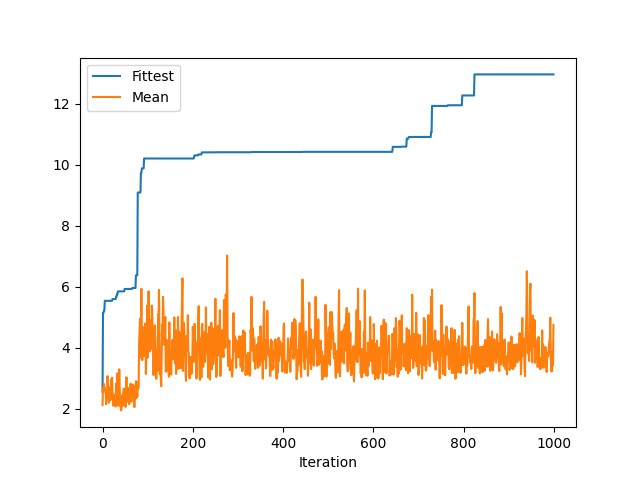
\includegraphics[width=8cm]{test1}
    \caption{First run of the GA}
    \label{fig:ga1}
\end{figure}

This iteration used 1000 generations with a population of 10 and 3 genes.

\paragraph{Iteration 2} In the second iteration, the mean fitness was actually lower than in the second iteration at around 3 units. But the overall fittest individual was found after around 200 generations at a fitness of around 12 units, after which major advancements were no longer found.

\begin{figure}[H]
    \centering
    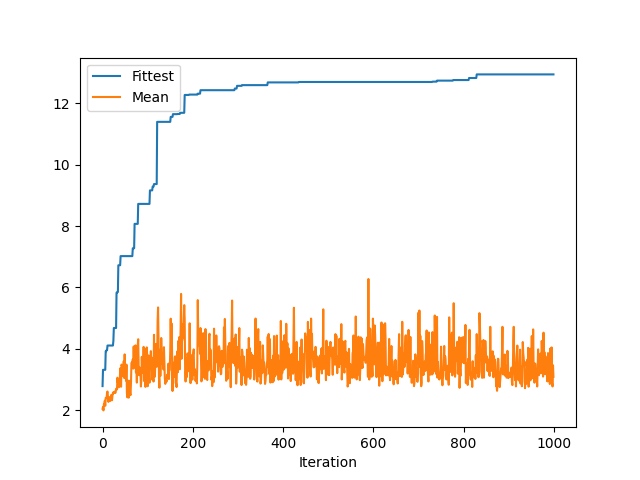
\includegraphics[width=8cm]{test2}
    \caption{Second run of the GA}
    \label{fig:ga2}
\end{figure}

\paragraph{Iteration 3} In the third iteration, the mean rose dramatically to about 25 units, while the fittest individuals were advanced after around 300 generations, when the fittest individual reached a fitness level of 300 units, and then exploded above 250 units after about 800 generations.

\begin{figure}[H]
    \centering
    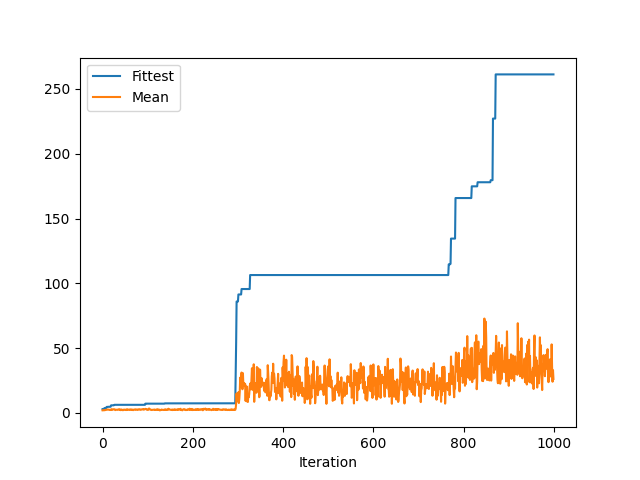
\includegraphics[width=8cm]{test3}
    \caption{Third run of the GA}
    \label{fig:ga3}
\end{figure}

\subsection{Experiment with the encoding scheme}

First I tried to manipulate the link length and shape by entering scaling values beyond 1 to observe what happens.

\begin{listing}[H]
    \caption{First change to encoding scheme}
    \begin{lstlisting}
"link-shape":{"scale":5}, 
"link-length": {"scale":5},
"link-radius": {"scale":5},
    \end{lstlisting}
\end{listing}


This yielded a fairly bulky creature that couldn't move very far.

\begin{figure}[H]
    \centering
    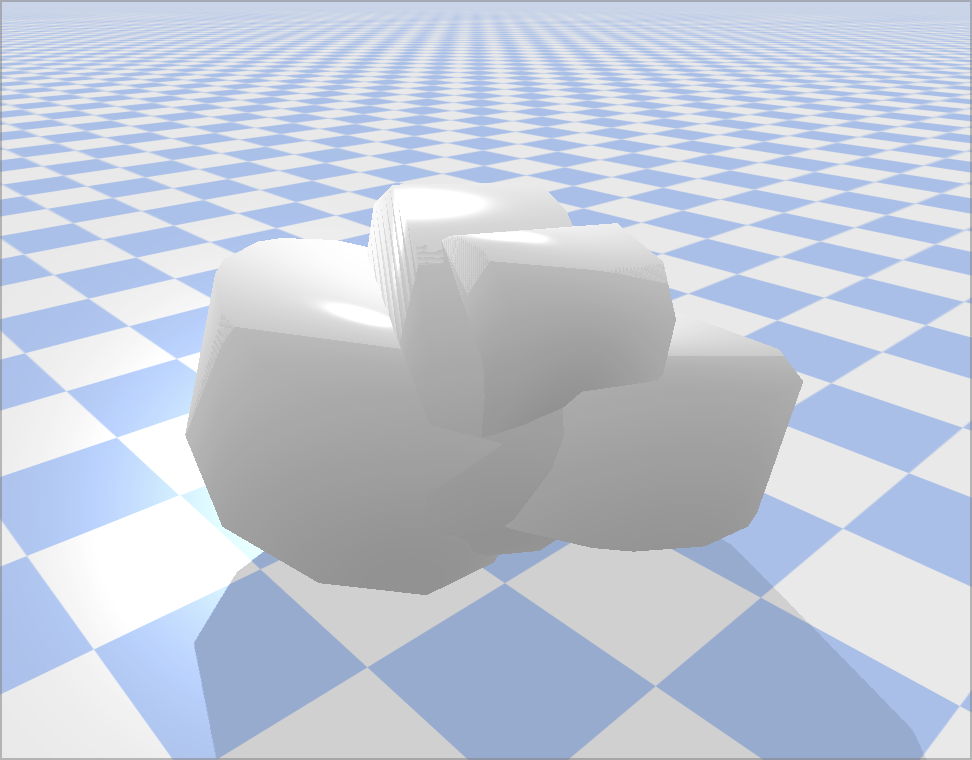
\includegraphics[width=8cm]{cr1}
    \caption{First change to encoding scheme}
    \label{fig:cr1}
\end{figure}


Next I tried to restrict the same parameters but also increased the link recurrence, hoping to generate more limbs that are spaced out and smaller.

\begin{listing}[H]
    \caption{Second change to encoding scheme}
    \begin{lstlisting}
{"link-shape":{"scale":0.5}, 
"link-length": {"scale":0.5},
"link-radius": {"scale":0.5},
"link-recurrence": {"scale":4}\end{lstlisting}
\end{listing}

This yielded a better creature with external, slender limbs that helped properl it forward slowly.

\begin{figure}[H]
    \centering
    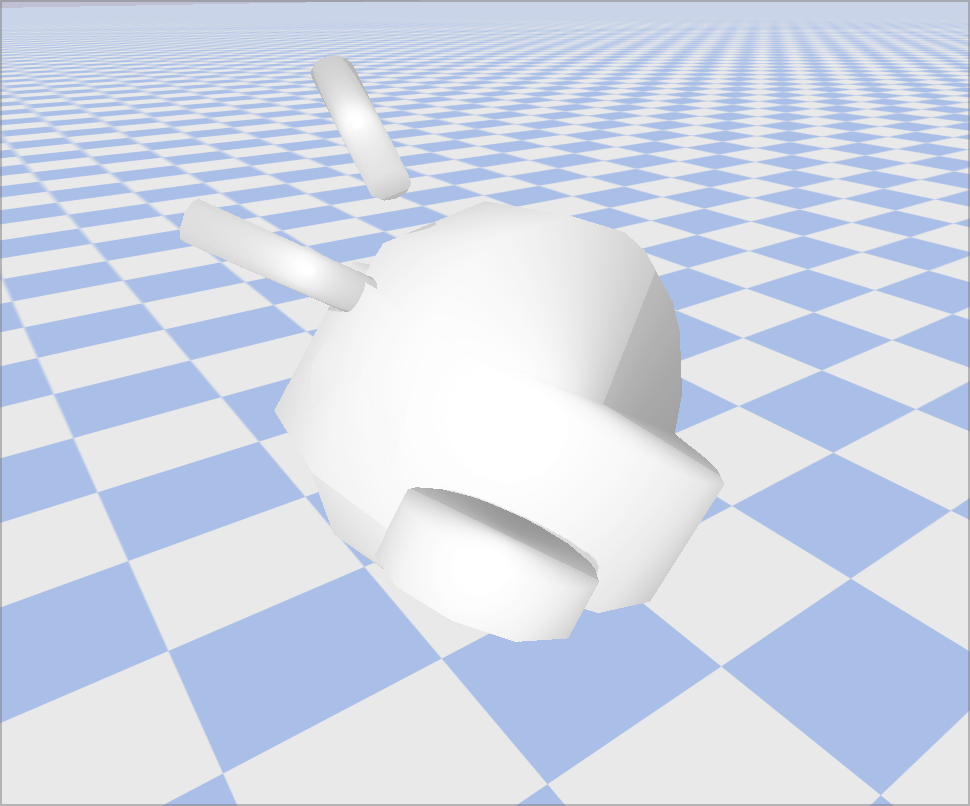
\includegraphics[width=8cm]{cr2}
    \caption{Second change to encoding scheme}
    \label{fig:cr2}
\end{figure}


Finally, I tried to manipulate the mass and joint patameters as well as the control waverform and frequency to generate different movement characteristics, such as more jolted movements.

\begin{listing}[H]
    \caption{Third change to encoding scheme}
    \begin{lstlisting}
{"link-shape":{"scale":0.5}, 
"link-length": {"scale":0.5},
"link-radius": {"scale":0.5},
"link-recurrence": {"scale":4}\end{lstlisting}
\end{listing}

This yielded a creature with only one external link but a rounder shape after 1000 generations; taking this version further with higher link recurrence might produce a fitter invidivual.

\begin{figure}[H]
    \centering
    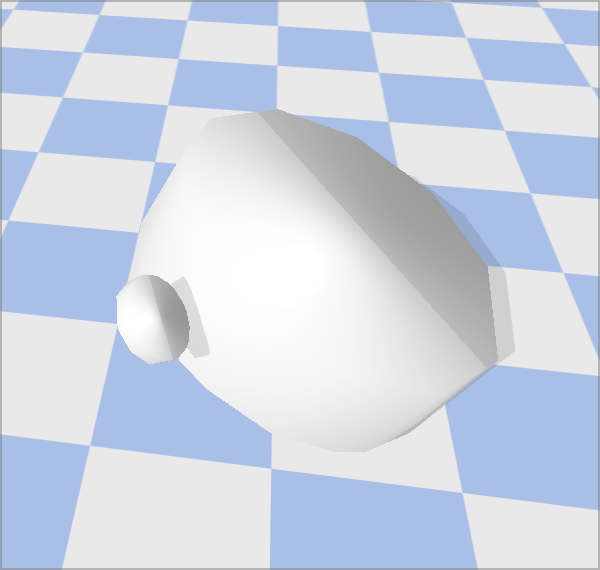
\includegraphics[width=8cm]{cr3}
    \caption{Third change to encoding scheme}
    \label{fig:cr3}
\end{figure}



\bibliographystyle{IEEEtran}
\bibliography{bib}


\end{document}